\scanpage{135}
Ci-dessus, on a \unsure{regardé|supposé} les coefficients \unsure{simples} \inserted{\unsure{finis}}, \uline{provenant de $k$}.

Regardons le cas des faisceaux de Weil \uline{concentrés} en un point $x\in C$. Alors \deleted{$\unsure{T(G)}\simeq$} [cas géom]
\[
T(G)\simeq G_x\quad\text{``considéré comme groupe algébrique sur $k$''}
\]
On doit prouver
\[
\operatorname{Ext}^i(C;\unsure{G_x|G},\deleted{\unsure{S}}\unsure{\sigma|\tau}\otimes\mu_n)\simeq
\operatorname{Ext}^{i-2}(k;G_x,\unsure{\sigma|\tau})
\]
Il est sans doute vrai que le $\operatorname{Ext}^i$ écrit est aussi le $\operatorname{Ext}^i$ \deleted{\uline{local}} fait \unsure{sur} le \unsure{hensélisé} de $\underline O_{C,x}\ldots$
\inserted{si $G=G_Y$ (où $Y=\{x\}$),}
\margin{$Y$ \unsure{partie fermée} finie de $C$}
\figure{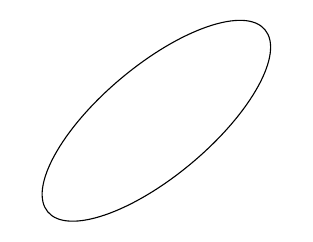
\begin{tikzpicture}\draw[rotate=40] (0,0) ellipse (1.8 and .7);\end{tikzpicture}}

Par la suite exacte des $\operatorname{Ext}$, on est ramené à \unsure{obtenir}
\deleted{$\operatorname{Ext}^*(C,G,\unsure{\sigma|\tau}\otimes\mu_n)\Longleftarrow H^p(C,\underline{\operatorname{Ext}}^q(G,\unsure{\sigma|\tau}\otimes\mu_n))$}
le th. de dualité, \deleted{\unsure{pour}} pour les \deleted{\unsure{G}} $i_!(F)$, i.e. : vérifions
\margin{$i:U\longrightarrow C$ est l'imm. \unsure{compl.} ($U=C-Y$)}
\figure{\begin{tikzpicture}[x=1cm,y=1cm]
\draw (-2,0) .. controls (-.8,.5) and (.8,-.5) .. (2,.2);
\draw (1.2,.2) .. controls (1,-.6) and (1.4,-1) .. (1.5,-.4) .. controls (1.6,-1.2) and (2,-1) .. (2.4,-.8);
\draw (1.1,-1) -- (2.6,-.9);
\end{tikzpicture}}
\[
\operatorname{Ext}^i(U;F,S\unsure{\sigma|\tau})\simeq
\operatorname{Ext}^{i}_{\unsure{\varphi|k}}(k;R\unsure{f_*}(\overset{\inserted{F_U}}{\overbrace{i_!F}}),\unsure{\sigma|\tau})
\]
où $\varphi_U:U\text{---}\operatorname{Spec}(k)$ est induit par $f\ldots$

\deleted{($F$ fini plat sur $U$) \unsure{premier à $p$}}

\unsure{\ensuremath{\omega})|a)} \deleted{$\unsure{F}$ \unsure{pour}} On est ramené à prouver que
\[
\boxed{H^{\unsure{i}}(U;\widehat F)\simeq\operatorname{Ext}^{i-2}(Rf_*(\deleted{\unsure{G}}F_U)),\mathbb Q/\mathbb Z)}
\]
\deleted{N.B. \unsure{bien distinguer}}\par
\deleted{\unsure{les groupes}}
\figure{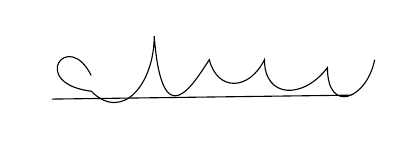
\begin{tikzpicture}[x=1cm,y=1cm]
\draw (0,.3) .. controls (-.3,.9) and (-.8,.2) .. (0,.1) .. controls (.4,-.3) and (.8,.2) .. (.8,.8) .. controls (.9,-.5) and (1.3,.2) .. (1.5,.5) .. controls (1.6,.1) and (2,.1) .. (2.2,.5) .. controls (2.2,0) and (2.7,0) .. (3,.4) .. controls (3,-.2) and (3.5,0) .. (3.6,.5);
\draw (-.5,0) -- (3.3,.05);
\end{tikzpicture}}
Ce qui définit une suite exacte (\unsure{déduite} de
$\unsure{0}\longrightarrow F_U\longrightarrow F\longrightarrow F_Y\longrightarrow0$
\deleted{$\operatorname{Ext}^{\unsure{i-2}}\longleftarrow$}
\diagram{\begin{tikzcd}[column sep=small]
\cdots & H^i(U;\widehat F) \arrow[l] & \operatorname{Ext}^{i-2}(Rf_*(F_{\unsure{Y}}),\mathbb Q/\mathbb Z) \arrow[l] & \operatorname{Ext}^{i-2}(Rf_*F_{\unsure{\cdot}},\mathbb Q/\mathbb Z) \arrow[l] & {}\arrow[l]
\end{tikzcd}}
on le vérifie par un calcul facile \deleted{\unsure{essentiel}}
(\unsure{n'utilisant} que les résultats de dualité déjà vérifiés\ldots) dans le cas où $F=\mu_n$ d'où $\widehat F=\mathbb Z/n\mathbb Z$,
($n$ \deleted{\unsure{quelconque}} \inserted{premier à $p\ldots$}), en \unsure{invoquant}, \deleted{\unsure{et ensuite}} [d'où \unsure{aussi},
\mspage{134}

